% !TeX spellcheck = en_EN-English

\section{Future record prediction}
\label{record_prediction}

This task is most important while also hardest to train. Our goal is to create model which would be able to predict potential next record based on patient previous ones. This task in general is almost impossible with amount of information we have, since there are many other factors that determine whether, when and what new disease will the patient become infected with in the future, whether his current state will improve or worsen, and most importantly what specific steps will doctor take.
\\

Fortunately our ultimate goal is not to predict specific patient future but only estimate how much would he most likely cost. So we expect that even though we wouldn't predict what exactly happens we would be able to estimate total cost of those records.
\\

We try multiple different model for this prediction. First three models we tried were recurrent neural networks (RNN). More specifically we tried multi-layer Elman RNN, multi-layered gated recurrent unit (GRU) RNN and multi-layer long short-term memory (LSTM) RNN. Last model we tried was Transformer.
\\

\subsection{Recurrent neural network}

In general recurrent neural network is type of neural network that in some way uses results from previous step or steps in order to improve prediction. These models are used for ordered data where next step is dependent on more than single previous one.

\subsection{Elman RNN}

Elman RNN also known as simple recurrent network (SNR) is type of recurrent neural network that utilize results of hidden layer before activation in previous step as an additional input in next one. We can see this architecture on figure \ref{fig:elman_arch}, where on left we can see how forward propagation look and on right how it looked unrolled over time, we see that middle layer which is a hidden layer of model gets two inputs, first is input vector $x_t$, where $t$ denotes step (usually time step), which is multiplied with matrix of weights $W_i$ and second one is vector $h_{t-1}$ which is result of this layer also called context vector in previous step. which is multiplied by different matrix of weight denoted as $W$, these two results after they are then summed together and result goes to activation layer which create resulting new vector $h_t$ \cite{elman}, this whole process can be summarized by this equation (where $b_i$ and $b$ are bias vectors):

\begin{equation}
	\label{eqn:elman}
	h_t = act(x_t W^T_i + b_i + h_{t-1} W^T + b)
\end{equation} 

Usually this result is directly used as output or go into single fully-connected feed-forward layer. In multi-layered version of this network, result of first hidden layer would go into next hidden layer together with result of that specific layer in previous step and again both would get multiplied by matrices of weight specific for that layer, summed and results goes through activation function.
\\

\begin{figure}[!h]
	\centering
	
	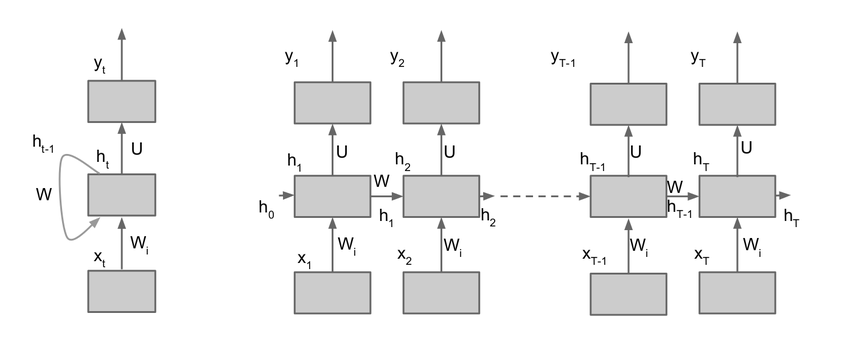
\includegraphics[width=0.85\textwidth]{images/Elman_RNN_architecture.png}
	
	\caption{Architecture of Elman RNN \cite{elman_img}}
	\label{fig:elman_arch}
\end{figure}

  

\subsection{Gated recurrent unit}
 
Gated recurrent unit is more complex recurrent neural network compared to Elman RNN. This model was developed as simplification of even more complex LSTM model. We can say that it consist mainly of three parts that interact with each other and together create final prediction. Those parts are reset gate, update gate and candidate hidden state computation. We can see structure of hidden layer of GRU on figure \ref{fig:gru_arch}. On this diagram sigmoid means fully-connected feed-forward layer with sigmoid activation function and tanh means fully-connected feed-forward layer with hyperbolic tangent activation function.
\\

Reset gate is on left side of diagram, it's task is to using input and previous hidden state vectors modify previous hidden state vector which goes into candidate hidden state computation. This should helps capture short-term dependencies in time series by removing part of information from previous hidden state vector.
\\

Candidate hidden vector computation is part that is similar to Elman RNN with two differences, firstly inputted hidden layer is modified by reset gate result and secondly resulting vector from this part is only candidate which goes into further calculation. This candidate contains mostly current and short-term past information thanks to specific vectors that input consist of. 
\\

Update gate, similarly to reset gate, uses concatenation of input and previous hidden state vector on input, but this time results are used to modify both previous hidden state and candidate hidden state in a way that resulting hidden state is weighted average of those two vectors where weights are results from this gate. This should help to capture long-term dependencies in time series from previous hidden state vector and reintroducing it into final hidden state by combining it with candidate hidden state vector that should contain mostly current and short-term information. 
\\ 

\begin{figure}[!h]
	\centering
	
	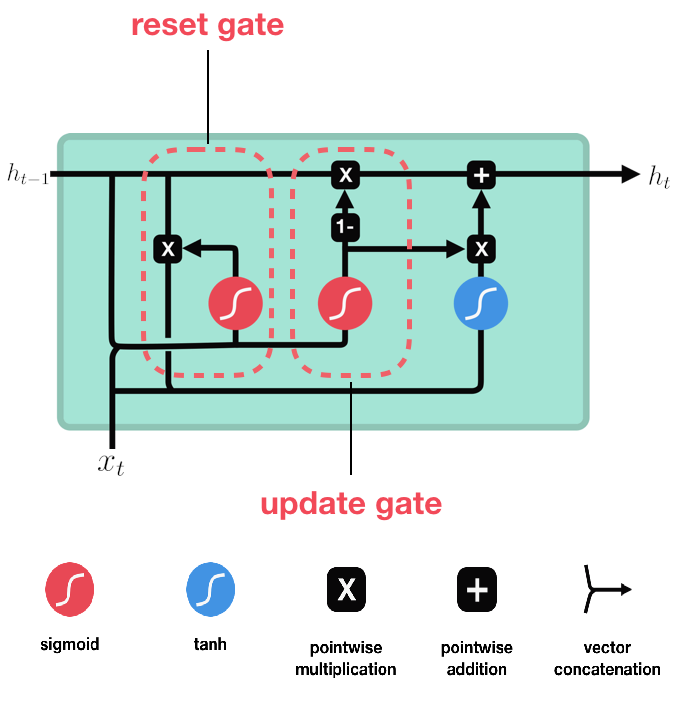
\includegraphics[width=0.6\textwidth]{images/GRU_arch.png}
	
	\caption{Architecture of GRU hidden layer}
	\label{fig:gru_arch}
\end{figure}
 
Multi-layered version is achieved by stacking hidden layers where hidden state vector of one layer is input vector of next one.
 
\subsection{Long short-term memory}

As mentioned earlier, long short-term memory is more complex predecessor of GRU. This model was developed with aim to mitigate vanishing gradient problem, that cause lack of long-term memory in models like Elman RNN, mainly by introducing memory vector, sometimes called memory cell, that should maintain information over longer period. As we can see in figure \ref{fig:lstm_arch} this model consist of three gates, candidate memory computation. Legend in this diagram have same meaning as one in GRU architecture diagram.
\\

All three gates and candidate memory computation has same input, which consist of input and previous hidden state vectors. In all of them this input goes into fully-connected feed-forward layer and then into activation function. In case of gates this activation function is sigmoid function, that bound all values into range (0,1), while candidate memory calculation uses hyperbolic tangent as activation function.
\\ 

Forget gate has the task of removing unnecessary information from memory vector by elementwise multiplication of it's result with previous memory vector. 
\\

Input gate together with candidate memory vector computation are meant to introduce new information into memory cell after adjustment from forget gate. Firstly model computes candidate memory then, then this vector is adjusted by input gate result and finally added to the modified previous memory vector. This results in new memory vector.
\\

Finally output gate is used to determine how much each part of memory should contribute into new hidden state vector.

 
\begin{figure}[!h]
	\centering
 	
	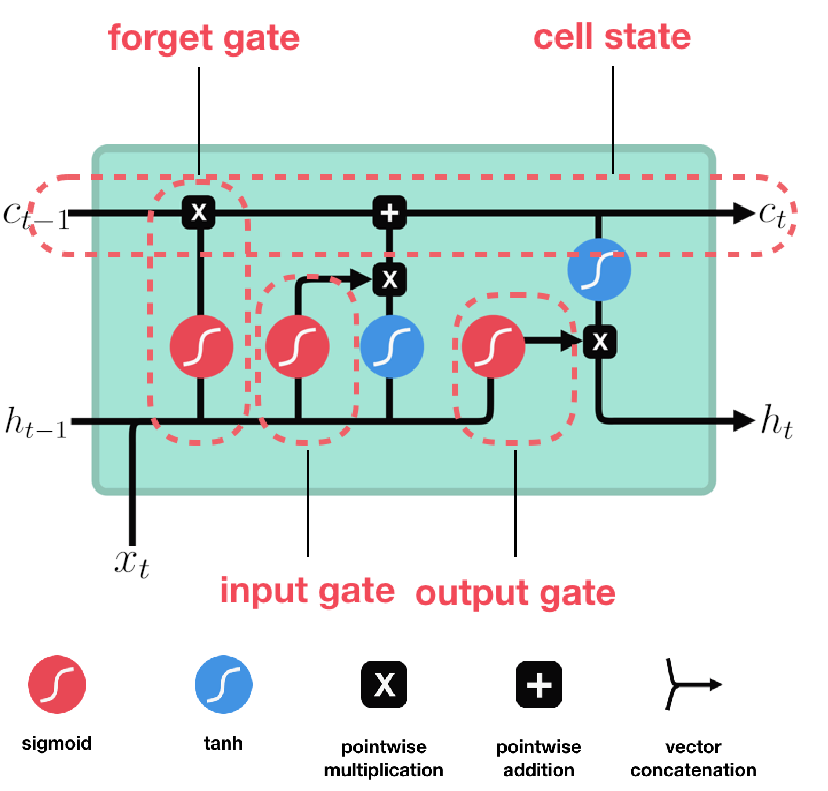
\includegraphics[width=0.6\textwidth]{images/LSTM_arch.png}
 	
 	\caption{Architecture of LSTM hidden layer}
 	\label{fig:lstm_arch}
\end{figure}

\subsection{Transformer}

Last tested model was transformer, compared to transformer explained in subsection \ref{emb:trans} here we tried more standard architecture that contains that contains both encoder and decoder shown in figure \ref{fig:trans}. Encoder in this model is meant to contextualized representation of input while decoder takes this contextualized representation and mixes together with previous outputs to get prediction of next output. Other than these two main blocks this model usually also contains tokenizer and embedding layer to prepare in going data and fully-connected feed-forward layer with softmax activation function to turn result of decoder into probability distribution of possible tokens.  
\\

\begin{figure}[!h]
	\centering
	
	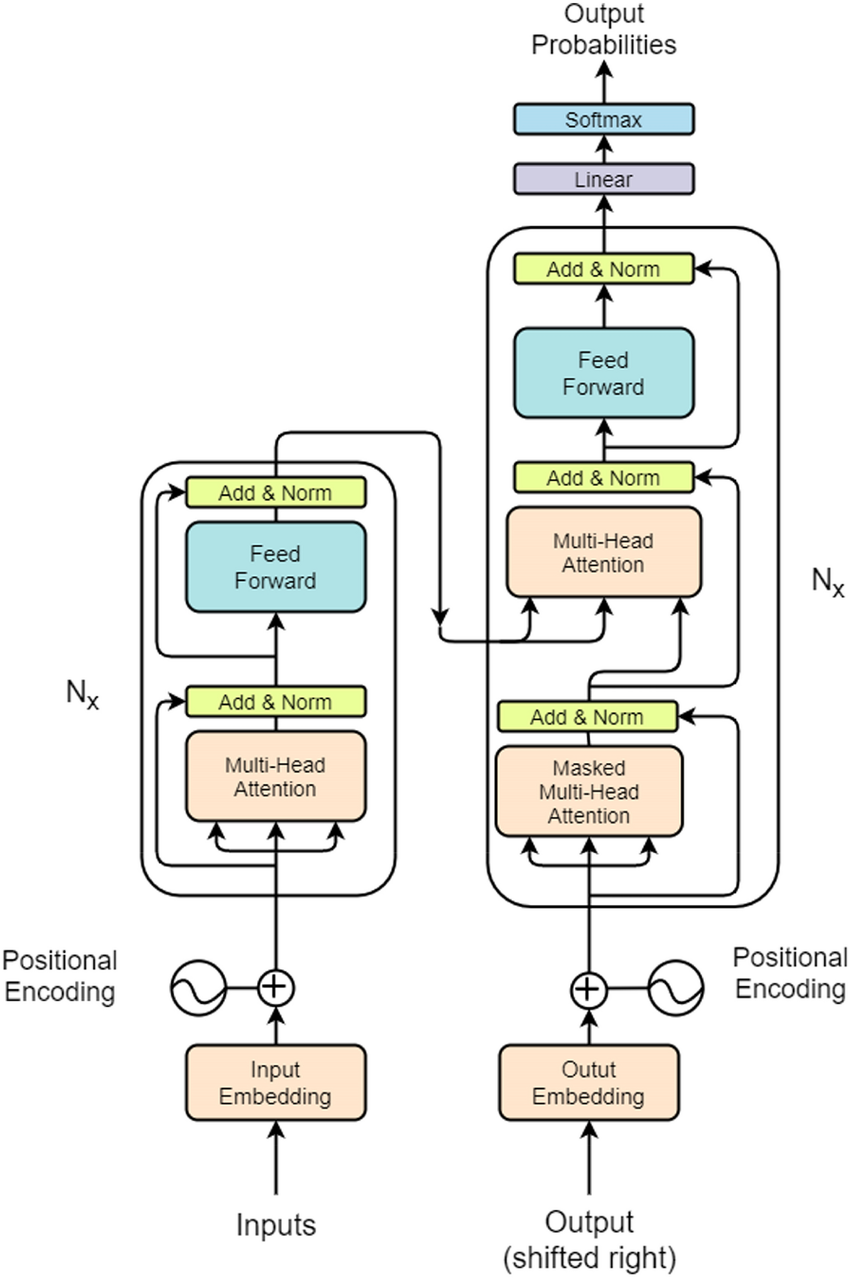
\includegraphics[width=0.6\textwidth]{images/trans_arch.png}
	
	\caption{Architecture of one encoder-decoder block in transformer model from original "Attention is all you need" paper \cite{attentionAllYouNeed}}
	\label{fig:trans}
\end{figure}

In our implementation we don't need tokenizer as our data are already in form of patient records which correspond to our tokens. In case of token embedding, we use embedding explained in section \ref{embedding} and we add positional encoding to make sure model take into account also order of records.
\\

Encoder architecture is very similar to one used in BERT and explained in \ref{emb:trans}, so it consist of multiple attention blocks where each block consist of multi-headed self-attention and multi-layered feed-forward neural network.
\\

Architecture of decoder, similarly to encoder, consist of multiple attention blocks, however in this case attention block consist of three parts instead of two. First is masked multi-headed self-attention which is similar to normal self-attention with only difference being application of masking to make sure that words on some specific positions does not affect words on other specific positions. Decoder use what's called casual or look-ahead masking which forbid future tokens to affect past ones, in our case this guarantees that record cannot be affected by record which happened after so in the future from it's perspective. Second part is multi-headed cross-attention, which takes two lists of token embeddings and compute effect of tokens in first list onto tokens in second list. In this case key and value vectors are computed from contextualized representation computed by encoder while query vectors are computed from results of self-attention in decoder. Final part of decoder attention block is multi-layered feed-forward neural network that further extract information from embeddings information from all attention heads. 
\\

After that results of decoder goes into final fully-connected feed-forward layer which change dimensionality of the decoder output from embedding size into vocabulary and apply softmax activation on result. This way we expect to get in last token probability distribution through all possible tokens. In our case we changed this last part. We run into problem where most of our records (our tokens) are unique creating extremely large vocabulary, this was caused partially by many possible combinations of disease, drug and medical procedure which are encoded in record and partially by timestamp which add additional uniqueness since it's improbable that two patients would get for example same drug, for same disease, at same age. Because of this we decided to remove softmax activation, changing fully-connected feed-forward layer in a way that result maintain dimension of embedding and added function that split result, find closest embedding of each part and concatenate result together leaving us with specific new embedding prediction instead of probability distribution.
\\

